\section{Intrinsic filtering for 2D manifold surface}

In this section, the detail of the intrinsic filtering model will be introduced for 2D manifold surfaces.
Furthermore, we explain that almost all classical filtering methods are special case of ours. %can be viewed as a simplification
And, we give an application to demonstrate the efficacy of our filter algorithm.

\subsection{Filtering for 2D manifold surface}

Suppose the signals we are interested in are defined on a 2D manifold surface $\Omega$ and with values in domain $\Gamma$.
Then the filtered signal $\bar{J_p}$ at point $p$ can be calculated by the following general form:
\begin{equation}
\label{Eq:GeneralForm}
\bar{J_{p}} = \frac{1}{W_{p}}\int_{\mathcal{N}(p)}\omega_{p, q}J_{q}d_{q}\, ,
\end{equation}
where, $J_{q}$ denotes the input signal at point $q$,
$\mathcal{N}(p)$ is the neighborhood of point $p$,
$\omega_{p, q}$ indicates the weight between $p$ and $q$,
and $W_{p} = \int_{\mathcal{N}(p)}\omega_{p, q}d_{q}$ is the normalization factor.% for ensuring the sum of all $\omega_{p,q}$ equal to 1.
For signal filter, the most important thing is how to construct $\omega_{p,q}$, since it directly relates to the performance of edge-preserving.

In the following, we define a weight which includes the cumulative difference of a path between two points $p$ and $q$:
\begin{equation}
\label{Eq:IntrinsicWeight}
\omega_{p,q} = g(d^{s}(\varphi_{p}, \varphi_{q}); \sigma_{s})g(d^{r}(\psi_p, \psi_q); \sigma_{r})\, ,
\end{equation}
where,  $g(\cdot \,; \cdot)$ is the kernel function.
We choose Gaussian function because it decreases quickly.
$\sigma_{s}$ and $\sigma_{r}$ are variance parameters.
$d^s$ and $d^r$ are defined as:
 \begin{equation}
 \label{Eq:IntrinsicDistance}
 \left \{
 \begin{array}{ll}
        d^{s}(\varphi_p, \varphi_q) = \lim_{\Delta{s}\to 0} (\int_{L}||\varphi_{q_{s + \Delta{s}}} - \varphi_{q_s}||^{n}ds\,\,)^{1/n} \vspace{1.5mm} \\
        d^{r}(\psi_p, \psi_q) = (\int_{L}||\psi_{s} - \psi_{p}||^{m}ds\,\,)^{1/m} \\
 \end{array}
 \right. .
 \end{equation}

Note that $L$ is the geodesic path between $p$ and $q$.
$\varphi$ and $\psi$ are two different signals, such as position, Gaussian curvature, and normal of a 2D manifold surface.
$q_{s + \Delta{s}}$, $q_s$ and $s$ are points on path $L$.

The cumulative differences $d^s$ and $d^r$ are able to reflect the local structure of desired signal.
The main reason is that the two cumulative differences are calculated on geodesic path and uses the signal difference.
According to different problems, we can choose suitable parameters $\varphi$, $\psi$, $n$ and $m$.

Equation \ref{Eq:IntrinsicDistance} can be approximated as:
 \begin{equation}
 \label{Eq:IntrinsicDiscreteDist}
 \left \{
 \begin{array}{ll}
        d^{s}(\varphi_p, \varphi_q) = (\sum_{q_{i+1}, q_i \in{L}}|\!|\varphi_{q_{i+1}} - \varphi_{q_i}|\!|^{n}|\!|q_{i+1} - q_{i}|\!|\,)^{1/n} \vspace{1.5mm}\\
        d^{r}(\psi_p, \psi_q) = (\sum_{q_{i+1}, q_i \in{L}}|\!|\psi_{q_i} - \psi_{p}|\!|^{m}|\!|q_{i+1} - q_{i}|\!|\,)^{1/m}
 \end{array}
 \right. .
 \end{equation}
In the above formula, $|\!|q_{i+1} - q_{i}|\!|$ is step length.
The orderly coordination of image can be regard as a discretization of 2D manifold.
And the step length is equal to 1 in image,
so according to our formulation, Bilateral filter[TM98], Geodesic filter[GS09], and image Propagation filter[CW15] are special cases of our model:

{\bfseries Case 1.}
Bilateral filter~\cite{tomasi1998bilateral}, as a classical nonlinear filter, uses two Gaussian functions as the spatial and range weights, respectively.
In our generalized model~\ref{Eq:IntrinsicDiscreteDist}, we use starting and end point $p$ and $q$ to replace the geodesic path $L$.
At the same time, signal functions $\varphi$ and $\psi$ are defined as $\varphi_{x} = x$ and $\psi_{x} = I_x$,
where $x$ is the pixel position and $I_x$ represents the pixel intensity.
When $m=2$ and $n=2$, our model is simplified as:
\begin{equation}
\label{Eq:BilateralDistance}
\left \{
\begin{array}{ll}
        d^{s}(p, q) = ||p - q|| \vspace{1.5mm}\\
        d^{r}(I_{p}, I_{q}) = || I_{p} - I_{q} || \\
\end{array}
\right. .
\end{equation}
We can see that the above formulation gets the distance differences, which are used to calculate the weights in bilateral filtering.

{\bfseries Case 2.}
Geodesic filter~\cite{grazzini2009edge} only uses $d^s$, one kind of accumulative difference in adjacent pixels during the process of image denoising.
This way gives a high response in image edges, so has a better edge-preserving power than bilateral filtering.
Setting $n=2$, the image intensity value $I$ as a signal value $\varphi$, and $d^{r}(\psi_p, \psi_q) = 1$,
our intrinsic filtering can be transformed into the following form:
 \begin{equation}
 \label{Eq:GeodesicDistance}
 \left \{
 \begin{array}{ll}
        d^{s}(I_p,I_q) = (\sum_{q_{i+1}, q_i \in{L}}||I_{q_{i+1}} - I_{q_i}||^{2}\,)^{1/2} \vspace{1.5mm} \\
        d^{r}(\psi_p, \psi_q) = 1 \\
 \end{array}
 \right. .
 \end{equation}

{\bfseries Case 3.}
In a similar way, our intrinsic filtering is simplified as a propagation image filtering~\cite{Chang2015propagated}
by setting $n=2$, $m=2$, $\varphi$ and $\psi$ both represent the pixel intensity.
Therefore,
 \begin{equation}
 \label{Eq:PropagationDistance}
 \left \{
 \begin{array}{ll}
        d^{s}(I_p, I_q) = (\sum_{q_{i+1}, q_i \in{L}}||I_{q_{i+1}} - I_{q_i}||^{2}\,)^{1/2} \vspace{1.5mm}\\
        d^{r}(I_p, I_q) = (\sum_{{q_i} \in{L}})||I_{q_i} - I_p||^2\,)^{1/2} \\
 \end{array}
 \right. .
 \end{equation}
Propagation filter \cite{Chang2015propagated} is a successful application of our method in image filtering.
\cite{Chang2015propagated} also demonstrates an outstanding power in preserving the image edge feature.


\begin{figure}
\centering
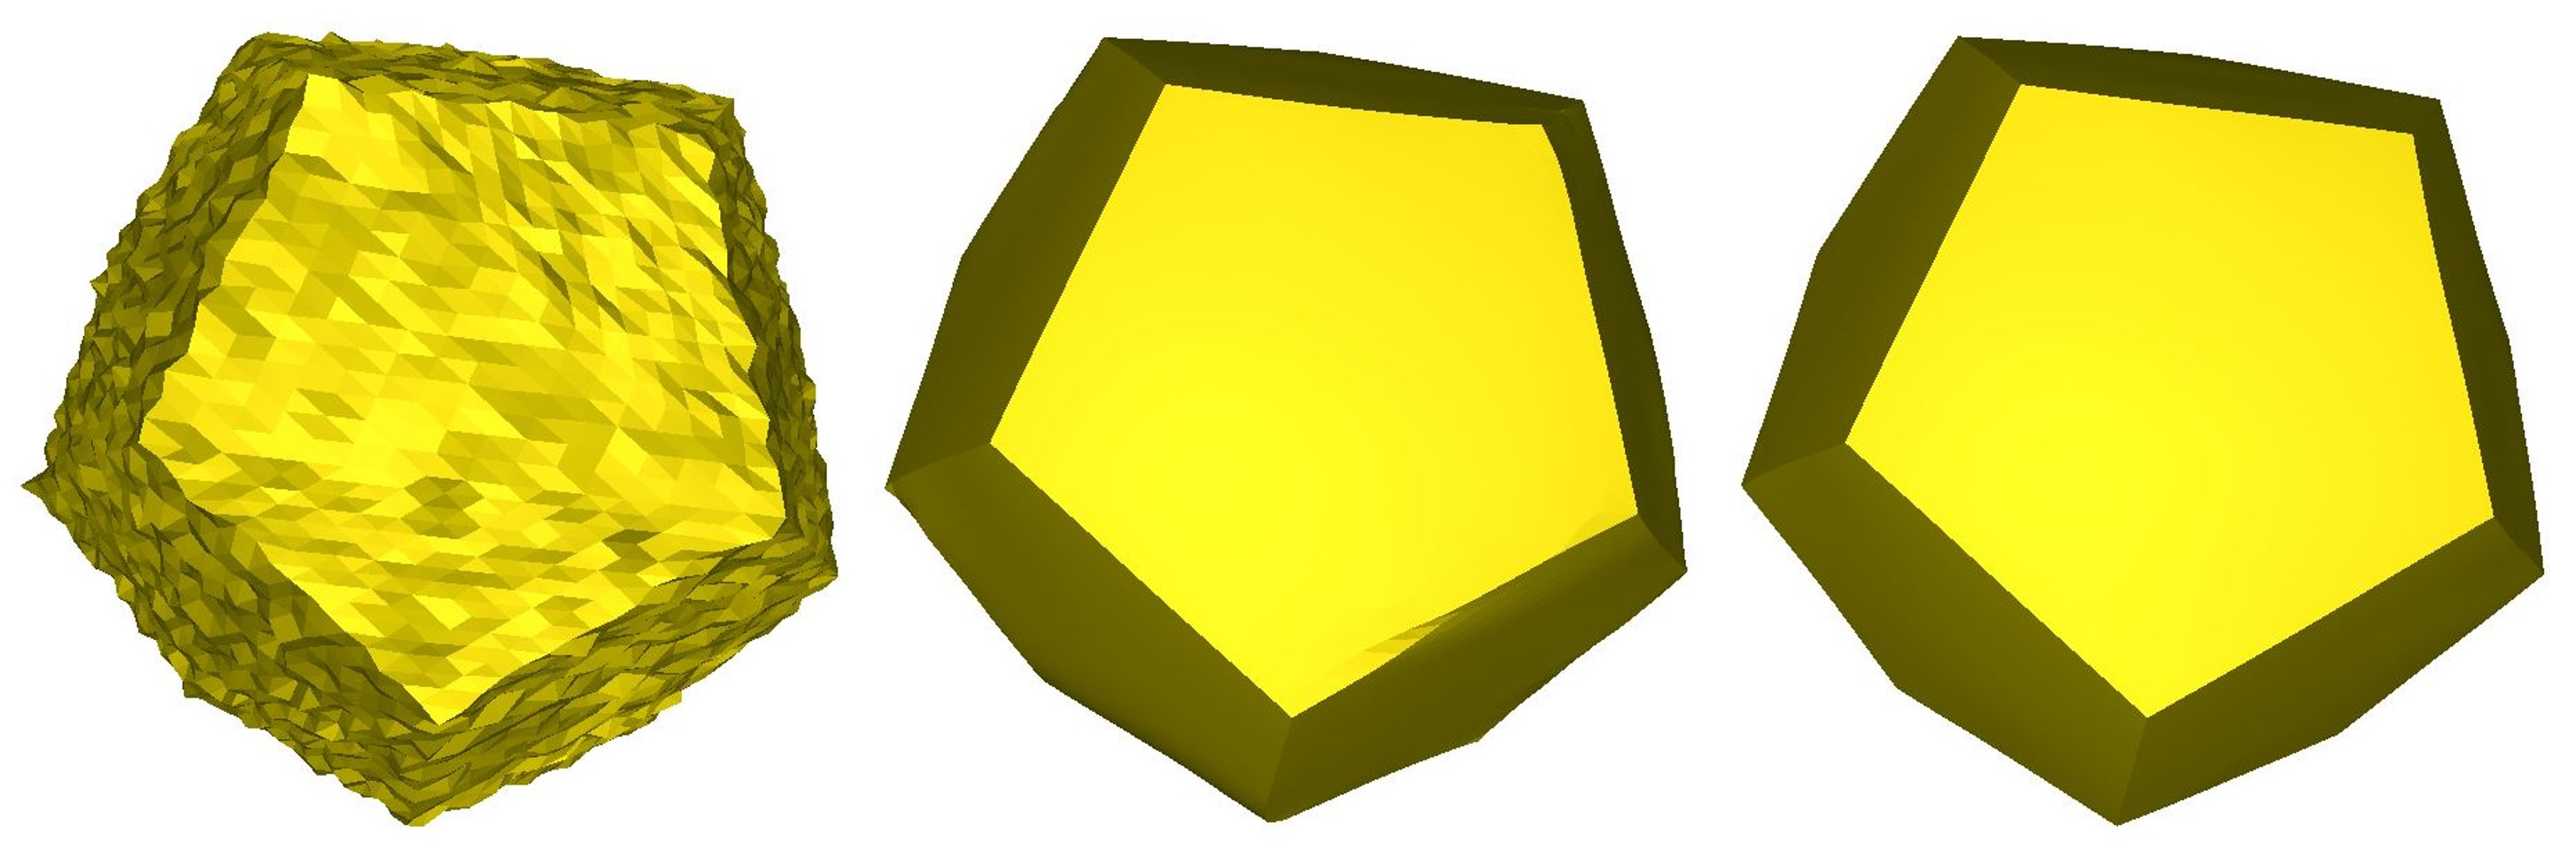
\includegraphics[width = 7.0cm]{results/shortest/shortest.jpg}
\vspace{-0.5mm}
\caption{ Comparison between geodesic paths and square-pattern paths. Left: the noisy mesh selected from~\cite{Wang2014decoupling}. Middle: the result of applying geodesic paths. Right: the result of applying square-pattern paths. The parameters of these two strategies are the same ($k_{iter} = 30$, $v_{iter} = 2$, $r = 4$, $\sigma_r = 0.3$ ). The time consumption is about 22.76s and 2.55s respectively. The former is not good in dealing with straight edges.}
\label{Fig:shortestpath}
\end{figure}

Our intrinsic filtering builds connections between $p$ and $q$, which providing more reliable information about the structure of the desired output.
And deciding the filtering weights is more reasonable and reliable.
Figure~\ref{Fig:relation} also shows this fact.
Further, we find our method inherits the advantage of these filtering algorithms~\cite{tomasi1998bilateral, grazzini2009edge, Chang2015propagated}, while compensating their deficiencies.


\subsection{Filtering mesh geometry}

Given a noisy triangle mesh, our goal is to filter the noise while keeping the mesh structures.
In order to achieve this purpose, we also adapt a two-stage process which be widely used in mesh filtering.
Firstly, noisy face normals are filtered iteratively by our intrinsic filtering model. %by equation~\ref{Eq:IntrinsicMeshFiltering}.
Secondly, according to the filtered face normals, vertex positions are updated.%iteratively though gradient descent.

{\bfseries Filtering face normals.}
When considering normals as a signal defined over the triangle mesh, it is easy to use the intrinsic filtering algorithm for mesh denoising.
First, the triangle face $f_{i}$ outward normal $\mathbf{n_{i}}$ can be easily calculated.
Then we consider $\mathbf{n_{i}}$ as a signal associated with the face barycenter $c_{i}$.
Next, we need find a path $L$ to connect $\mathbf{n_{i}}$ and its neighbor $\mathbf{n_{j}}$.
In order to filter the face normals $\mathbf{n_{i}}$, we need find a path $L$ to connect $\mathbf{n_{i}}$ and its neighbor $\mathbf{n_{j}}$.
Finally, a filtered face normal $\bar{\mathbf{n_{i}}}$ is computed through our intrinsic mesh filtering model:
 \begin{equation}
 \label{Eq:IntrinsicMeshFiltering}
 \bar{\mathbf{n_{i}}} = \frac{1}{W_{i}}\sum_{\mathclap{f_{j}\in\mathcal{N}_{i}}}A_{j}g(d^{s}(\mathbf{n_{i}}, \mathbf{n_{j}}); \sigma_{s})g(d^{r}(\mathbf{n_{i}}, \mathbf{n_{j}}); \sigma_{r})\mathbf{n_{j}}\, .
 \end{equation}
  here,
 \begin{equation}
 \label{eq:IntrinsicMeshDistance}
 \left \{
 \begin{array}{ll}
        d^{s}(\mathbf{n_{i}}, \mathbf{n_{j}}) = (\sum_{x, x+1\in{L}}||\mathbf{n_{x+1}}-\mathbf{n_{x}}||^{n}\,\,)^{1/n} \vspace{1.5mm} \\
        d^{r}(\mathbf{n_{i}}, \mathbf{n_{j}}) = (\sum_{x\in{L}}||\mathbf{n_{x}}-\mathbf{n_{i}}||^{m}\,\,)^{1/m} \\
 \end{array}
 \right. ,
 \end{equation}
where, $W_{i}$ is the normalization factor,
calculated by
$||\sum\limits_{\mathclap{f_{j}\in\mathcal{N}_{i}}}A_{j}g(d^{a}(\mathbf{n_{i}}, \mathbf{n_{j}}); \sigma_{s})g(d^{r}(\mathbf{n_{i}}, \mathbf{n_{j}}); \sigma_{r})||$
which ensures that $\bar{\mathbf{n_{i}}}$ is a unit normal;
$A_j$ is the area of $f_j$;
$\mathcal{N}_{i}$ is the neighborhood of $f_{i}$.
In our paper, we use the geometrical neighborhood, defined in~\cite{Zhang2015Filter}.

Note that, equation \ref{Eq:IntrinsicMeshFiltering} can be derived from equation \ref{Eq:GeneralForm}.
$A_j$ is the accumulation of infinitesimal area because the domain of integration is triangle face.
Furthermore, we give up the step length which measures the distance between adjacent barycenter of triangle faces. % to facilitate the calculation in equation \ref{eq:IntrinsicMeshDistance}.
We simply set it to one for facilitating the calculation.

Although the geodesic algorithm gives the shortest distance between two points, its calculation is expensive.
To improve computational efficiency, we introduce a simple, fast and effective strategy to chose filtering paths, which will be in the next section.
In Figure \ref{Fig:shortestpath}, we compare the calculation efficiency and results obtained by these two strategies.
The proposed strategy is much faster than geodesic distance.
Furthermore, the result obtained by our strategy is much better in dealing with details, like edges and corners.

\begin{figure}%[htb]
\centering
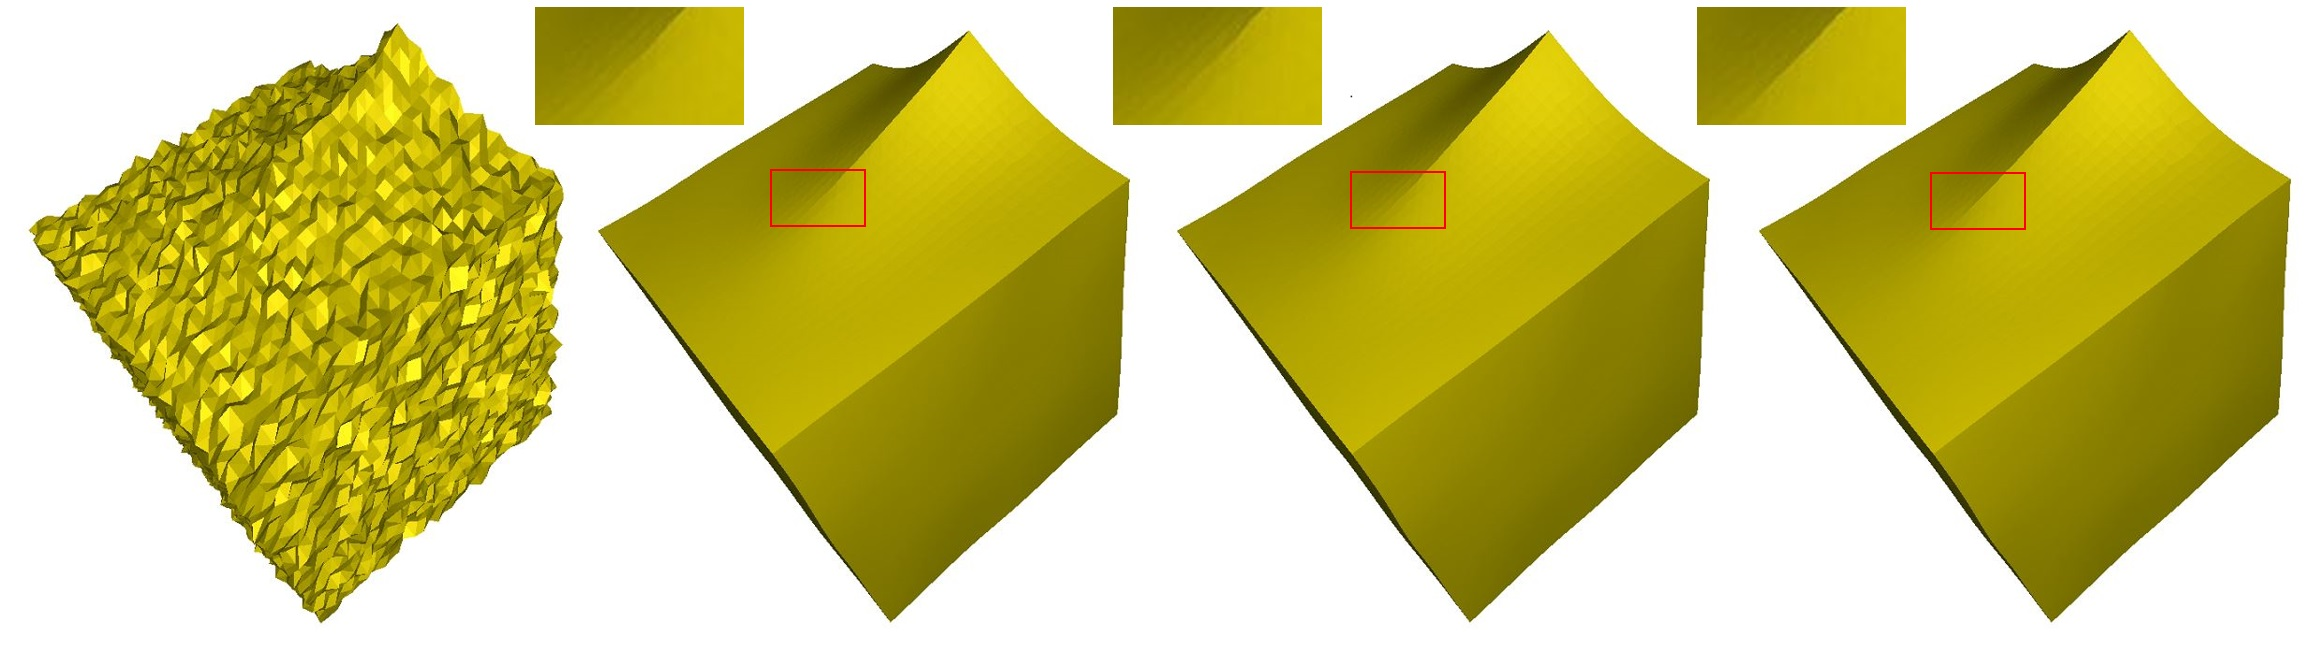
\includegraphics[width = 7.5cm]{results/Norm/norm.jpg}
\vspace{0.5mm}
\caption{ From the left to right: Noised mesh ( Gaussian noise with 0.3$\sigma_E$ ), the results of $m = n = 2$ with step length,
$m = n = 2$ without step length, $m = n = 1$ without step length.
Because of the sparseness of mesh feature, $L_1$ norm receives the best results in preserving the mesh structure.}
\label{Fig:norm}
\end{figure}

\begin{figure}
\centering
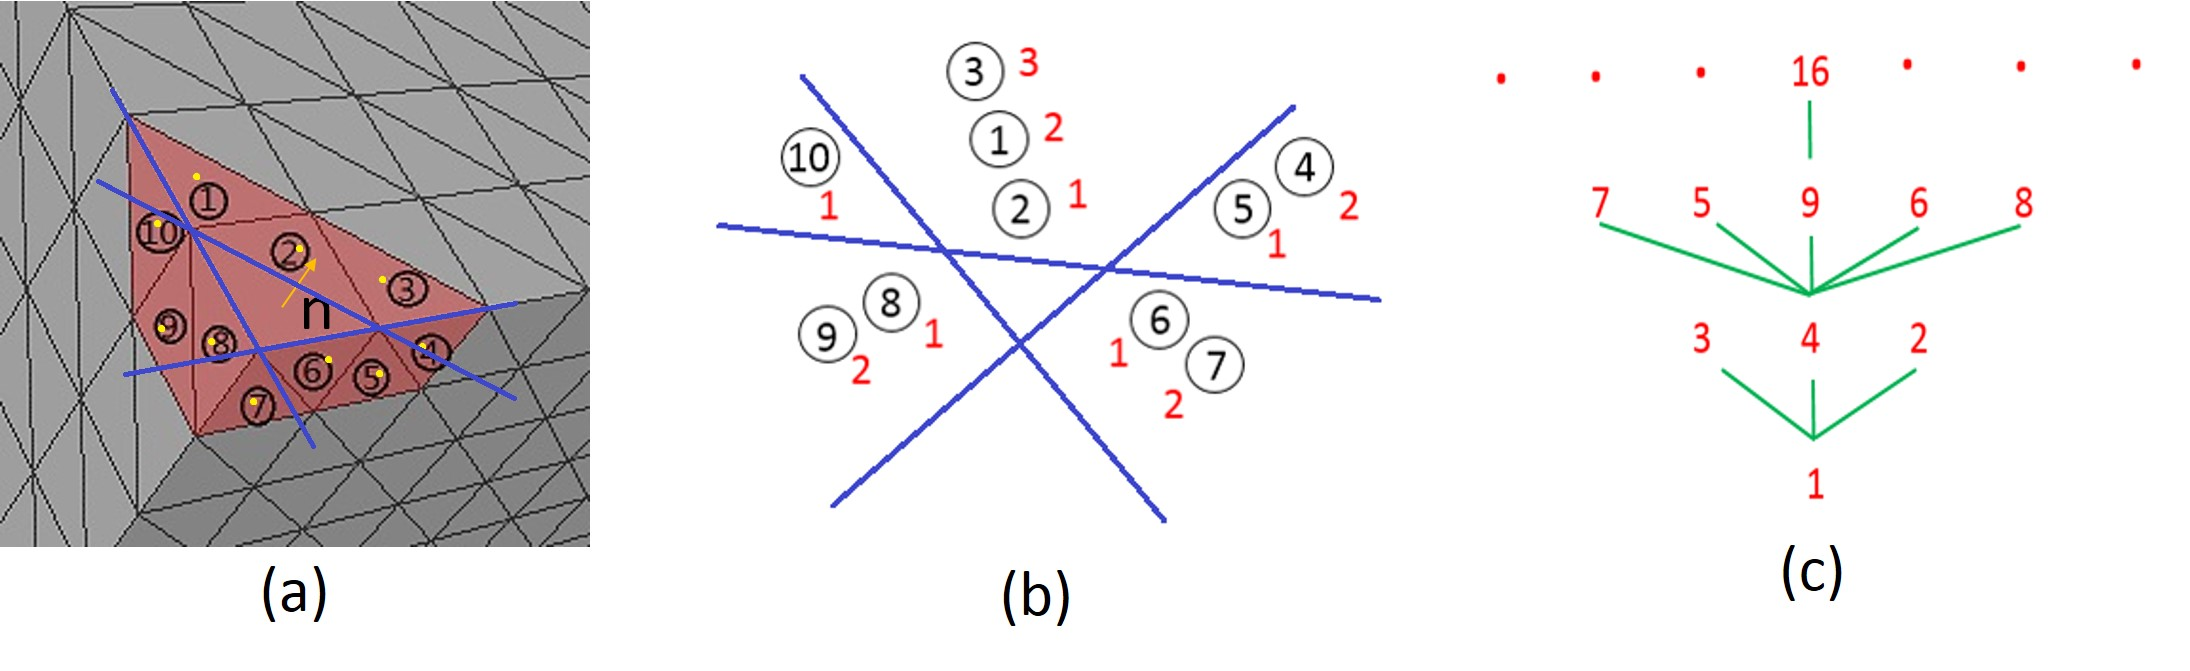
\includegraphics[width = 7.5cm]{results/Path/path1.jpg}
\vspace{-3mm}
\caption{ The process of generation path. (a) the 10 neighbors of current face with its normal $\mathbf{n}$. (b) The schematic diagram after projection, dividing and sorting. (c) the pattern.
The numbers with circle are the neighbor of current triangle face, the yellow points are the projection points of neighbor face centroid, the blue lines are used to decide the face label, the red numbers are their serial number after sorting, the green lines are connected path.}
\label{Fig:path}
\end{figure}

To chose appropriate m and n,  we conduct several experiments.
Figure~\ref{Fig:norm} shows the experimental results.
From this figure we can see that both m and n are set to 1 can obtain the best result, since features on 3D meshes are always sparse.

 {\bfseries Updating vertices.} After all face normals are filtered, the vertex positions need to be updated to cater to these new normals.
 We adopt the iterative scheme in the paper~\cite{sun2007fast} to update the vertex positions.
 Namely, for a face $f_{i}$, its vertex positions are updated via the following iteration form
 \begin{equation}
 \label{vertexupdate}
 \bar{v_{i}}^{(t+1)} = \bar{v_{i}}^{(t)} + \frac{1}{|{\mathcal{F}_{i}}|}\sum_{j\in\mathcal{F}_{i}}\mathbf{\bar{n}_{j}}[\mathbf{\bar{n}_{j}}\cdot(\bar{c_{j}}^{(t)}-\bar{v_{j}}^{(t)})]\, ,
 \end{equation}
 where, $\bar{v_{j}}^{(t)}$ is the value of $\bar{v_{i}}$ in the $t-th$ iteration,
 $\mathcal{F}_{i}$ is the index set of the incident faces for $\bar{v_{i}}$,
 $|\cdot|$ denotes the cardinality of a set,
 and $\bar{c_{j}}^{(t)} = \sum_{i=1}^{3}\bar{v_{j_{i}}}^{(t)}/3$ is the barycenter of the triangle $f_{j}$.
 Gradient descend process can be used to solve this formulation.
% This scheme is actually based on the orthogonality between the normal and the three edges of each face on the mesh.
% Then adopts a gradient descend process for solving that orthogonality equation in the conditions of  $L_2$ error.

 In our experiments, almost all models need less than 75 iterations to achieve satisfactory results for filtering face normals,
 and approximately up to above conditions about 5 iteration in the process of vertex update.
 %10 to 20 iterations are sufficient for achieving satisfactory results
 %and approximately up to above conditions.
 Pseudocode of our mesh filter algorithm is shown in Algorithm~\ref{alg:1}.
 In the next section, we will solve the problem in selecting filter path.


\begin{algorithm}\caption{Intrinsic mesh filtering framework}
\label{alg:1}
\begin{algorithmic}
\STATE {\textbf{Input:} Initial mesh $M_{in}$, number of iterations $k_{iter}$.}
\STATE{\textbf{Output:} Filtered mesh $M_{out}$.}
\STATE{1: $M^{(0)} = M_{in}$}
\STATE{2: Compute the path sets $\mathcal{P}$} according to section \ref{Sec:path}.
\STATE{3: \textbf{for} $s = 1$ to $k_{iter}$ \textbf{do}}
\STATE{4: ~~~Compute face normals {$n_i$} of mesh $M^{(s-1)}$;}
\STATE{5: ~~~Get the paths {$\mathcal{P}_i$} of {$n_i$};}
\STATE{6: ~~~Compute filtered normals {$\mathbf{\bar{n_i}}$} according to~\ref{Eq:IntrinsicMeshFiltering};}
\STATE{7: ~~~Compute updated mesh $M^{(s)}$ according to {$\mathbf{\bar{n_i}}$};}
\STATE{8: \textbf{end for}}
\STATE{9: $M_{out} = M^{k_{iter}}$.}
\end{algorithmic}
\end{algorithm}



 \section{Path chosen for mesh filtering}
 \label{Sec:path}


 For an image, many particular patterns can be chosen because of the regular coordination system.
 These patterns are simple and easy to be thought about.
 But for a triangle mesh, it is very difficult to obtain a good pattern which can preserve the mesh feature.
 The easiest way is to use geodesic distance defined on triangle mesh.%to be thought of is applying the shortest path algorithm on the triangle mesh.
 However, as seen in figure \ref{Fig:shortestpath}, this method is time consuming.
 %We solve this problem in this paper within the context of mesh denoising.

To solve this problem, we propose a simple strategy to chose path.
 Our method is based on the following theory: the areal coordinates of triangles segment the plane into seven regions.
 Areal coordinates are extremely useful in engineering applications involving triangular subdomains.
 These make analytic integrals often easier to evaluate, and Gaussian quadrature tables are often presented in terms of area coordinates.
 In the context of triangle, the areal coordinates of a point $P$ are the ratios of the areas of $PBC$, $PCA$ and $PAB$ to the area of the reference triangle $ABC$.
 %shown in the figure~\ref{Fig:path}(a).
 Because the ratios are a plus or a minus, it divide the plane where the triangle is to seven parts.
 That gives us an enlightenment to obtain a particular pattern for solving the problem of paths.

{\bfseries Path generation.}
For each triangle $f_i$, we project its neighborhood $\mathcal{N}_i$ onto a tangent plane based on its normal $\mathbf{\bar{n_i}}$.
In practice, we only project their barycenter onto that plane.
Then basing the three points of $f_i$, we use areal coordinations to divide these barycenters to seven regions.
Note that, if the projection point falls into the face $f_i$, we throw it away from $\mathcal{N}_i$.
In this way, we give each neighbor a label that belong to a specified region.
Afterwards, we sort these neighbors belong to the same region according to their face barycenter distance to $c_i$ in original noisy mesh.
Finally, we provide a particular pattern to assign the path for matching the ordered neighbors.
This pattern is defined square-pattern, which is used for generating paths.
The entire process is depicted in the figure~\ref{Fig:path}.

{\bfseries Advantages.}
 The above process has the power to protect local mesh features, such as edges and corners.
 To a certain extend, the six regions surrounding $f_i$ depict the local structure of a mesh.
 Projecting along the normal of $f_i$ makes the faces having similar normal flock together.
 Furthermore, the division further restricts the normal difference according to areal coordinates.
 The combination of these two aspects insures that one of six regions has the similar normal to $f_i$.
 The part including faces $\textcircled{1}$, $\textcircled{2}$ and $\textcircled{3}$ has the similar normal to $f_i$ in the figure \ref{Fig:path}(b).
 These normals play a important role in applying our intrinsic filtering algorithm.

 Figure \ref{Fig:path}(c) shows the square-pattern for generating path.
 We use $n^2$($ n = 1, 2,...$) as connection points, the sequence numbers between $(m-1)^2$ and $m^2$ including $m^2$ directly connect the number $(m-1)^2$.
 In this way, paths are generated.
 For example, the path between number $8$ and $f_i$ is $8-4-1-f_i$, number $16$ and $f_i$ is $16-9-4-1-f_i$ and so on.
 Once generating the paths, they will not change in the subsequent iterations.

 In the next section, we will introduce the experimental results basing our method.
